%sensory systems generally
The sensory systems of brains do remarkable work in extracting behaviorally useful information from noisy and complex raw sense data. 
Vision systems process intensities from retinal photoreceptor arrays, auditory systems interpret the amplitudes and frequencies of hair-cell displacements, and somatosensory systems integrate data from direct physical interactions.~\cite{purves2001neuroscience} 
While these systems differ radically in their input modalities, total number neurons, and specific neuronal microcircuits, they share two fundamental characteristics. 
First, they are hierarchical sensory cascades, albeit with extensive feedback, consisting of sequential processing stages that together produce a complex transformation of the input data.  
Second, they operate in inherently highly-structured spatiotemporal domains, and are generally organized in maps that reflect this structure~\cite{felleman1991distributed}.

Extensive experimental work in the rodent whisker-trigeminal system has provided insights into how these principles help rodents use their whiskers (also known as \emph{vibrissae}) to tactually explore objects in their environment.  
Similar to the ventral stream of visual systems with hierarchical structures from V1, to V2, V4, and IT~\cite{felleman1991distributed, Goodale1992, Diamond2008, yu, moore, dosman, bensmaia}, researchers have found evidence of hierarchical processing for somatosensory input in rodents, human, and primates\cite{Pons1987, Inui2004, Iwamura1998}. 
Information from the whiskers is relayed from primary sensory neurons in the trigeminal ganglion --- each of which responds to multiple trigeminal nuclei, which form the origin for multiple parallel pathways conveying information to thalamus and then primary somatosensory cortex (S1).
Secondary somatosensory cortex (S2) is found to rely on inputs from S1 (first somatosensory area) \cite{Pons1987, Petersen2007}. 
Barrel cortex, S1, and S2 accept input from subcortical cascade driven by  whiskers input \cite{Diamond2008}. 
However, although the rodent somatosensory system has been the subject of extensive experimental efforts, there have been comparatively few attempts at computational modeling of this important sensory area. 

Recent work has shown that deep neural networks (DNNs), whose architectures inherently contain, can be effective models of neural processing in vision\cite{} and audition\cite{}.
Motivated by these successes and by the known structure of rodent barrel cortex, in this work we illustrate initial steps toward using DNNs to model rodent somatosensory systems.
Our driving hypothesis is that rodent barrel cortex is optimized to use whisker-based sensor data to solve somatosensory tasks in complex, variable real-world environments. 
The basic idea in our approach is thus to use \emph{goal-driven} modeling (Fig \ref{fig_schematic}), in which the DNN parameters --- both discrete and continuous --- are optimized for performance on a challenging ethologically-relevant task\cite{}.  
Insofar as the shape recognition task is a strong constraint on network parameters, the resulting optimized neural network may be an effective model of real barrel cortex neural response patterns. 
 
\begin{figure}
\centering
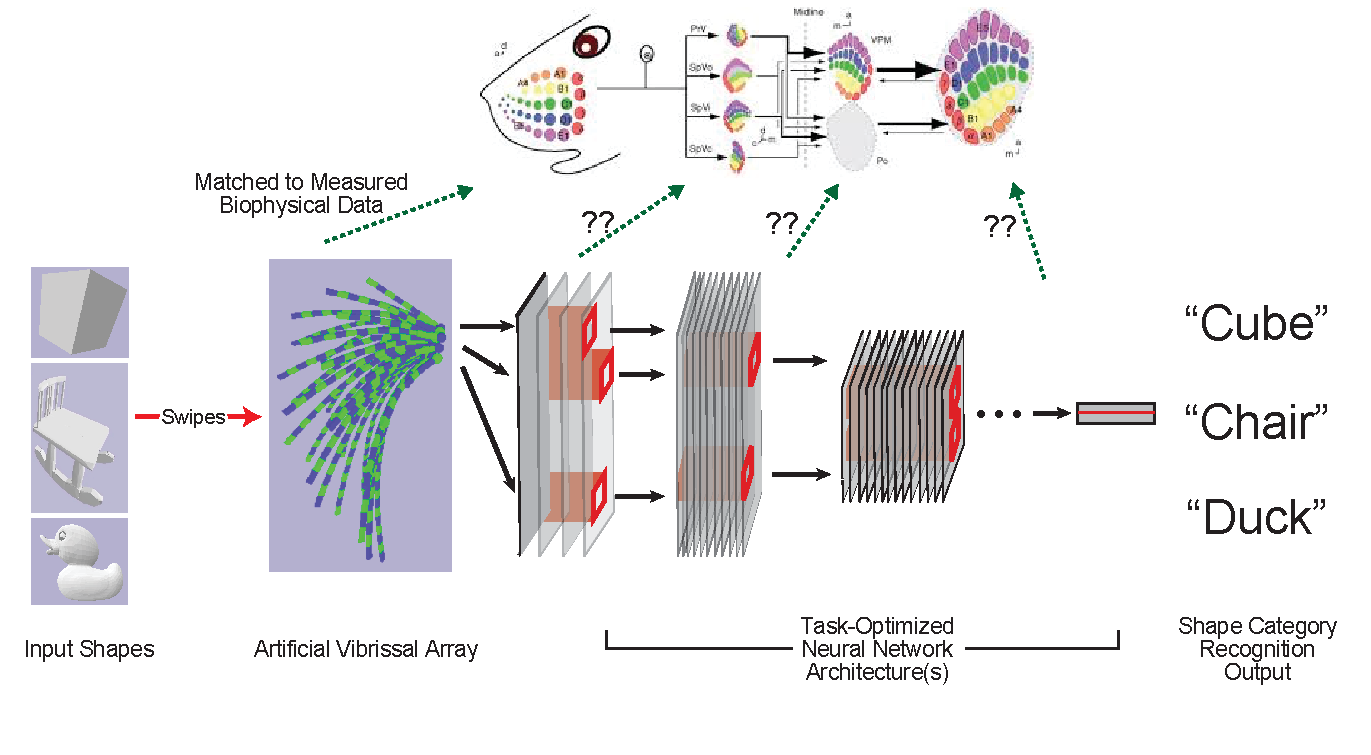
\includegraphics [width=1\linewidth]{figures/schematic.pdf}
\vspace{-2mm}
\caption{\textbf{Goal-Driven Approach to Modeling Barrel Cortex:} \textbf{a.} Rodents have highly sensitive whisker arrays that provide input data about the animal's environment.  Whisker signals are is subsequently processed by a somatosensory cascade of brain areas knowns as barrel cortex. Barrel cortex is a prime target for modeling because it is likely to be richly representational, but its computational underpinnings are largely unknown. Our long-term approach to modeling barrel cortex is \emph{goal-driven}: using an artificial whisker-array input device built using extensive biophysical measurements (\textbf{b.}), we seek to optimize neural networks of various architectures (\textbf{c.}) to solve ethologically-relevant shape recognition tasks (\textbf{d.}), and then measure to what extent the networks predict fine-grained response patterns in real neural recordings. ~\label{fig_schematic}}
\end{figure}

This idea is conceptually straightforward, but implementing it involves surmounting several major challenges.  
Unlike the cases of vision or audition, where the contents of the retina or cochlea can for many purposes be approximated by a mathematically simple data array (namely, a uniform data array representing light or sound intensities), the equivalent mapping between stimuli (e.g. objects in a scene) and the sensor input to the whisker system is much less direct.   
Thus, a biophysically-realistic embodied model of the whisker array is a critical first component of any barrel cortex model.
Once the sensor is available, a second key problem is building a neural network that can accept whisker data input and use it solve relevant tasks. 
Aside from the question of the neural network design itself, knowing what the ``relevant tasks'' are for training a rodent whisker system, in a way that is sufficiently concrete to be practically actionable, is a significant unknown, given the very limited amount of ethologically-relevant behavioral data on rodent sensory capacities\cite{}.
Collecting neural data of sufficient coverage and resolution to quantitatively evaluate one or more task-optimized neural network models represents a third major challenge.   

In this work, we show initial steps on the first two of these problems (sensor modeling and neural network design/training). 



